\documentclass{beamer}
\usepackage{../../shared/styles/custom}
\usepackage{../../shared/styles/conventions}

\usepackage{grffile}

\title{Lasso Regression}
\date{\today}
\author{Nipun Batra}
\institute{IIT Gandhinagar}
\begin{document}
  \maketitle
  
\begin{frame}{Lasso Regression}
\begin{itemize}[<+->]
	
	
	\item LASSO $\longrightarrow$ Least absolute shrinkage and selection operator
	\item Popular as it leads to a sparse solution.
	
\end{itemize}
\end{frame}

\begin{frame}{Constructing the Objective Function}
\begin{itemize}[<+->]

\item Find a $\vtheta_{\text{opt}}$ such that  \begin{equation}    \vtheta_{\text{opt}} =  \argmin_{\vtheta} {(\vy-\mX\vtheta)^T(\vy-\mX\vtheta)} : \ ||\vtheta||_1<s \end{equation}
\item Using KKT conditions
\begin{equation}
    \vtheta_{\text{opt}} = \underbrace{\argmin_{\vtheta}{(\vy-\mX\vtheta)^T(\vy-\mX\vtheta) + \delta^2||\vtheta||_1}}_\text{convex function}
\end{equation}
	
\end{itemize}


\end{frame}

\begin{frame}{Solving the Objective}
\begin{itemize}[<+->]

\item Since $||\vtheta||_1$ is not differentiable, we cannot solve,  \begin{equation}    \frac{\partial {(\vy-\mX\vtheta)^T(\vy-\mX\vtheta) + \delta^2||\vtheta||_1}}{\partial \vtheta} = 0 \end{equation}

\item How to Solve?
Use coordinate descent!
\end{itemize}

\end{frame}

\begin{frame}{Sample Dataset}

\begin{figure}
    \centering
    \includegraphics[scale = 0.75]{../assets/lasso-regression/figures/true_function.pdf}
    \caption{y = 4x + 7}
    \label{fig:my_label}
\end{figure}{}

\end{frame}

\begin{frame}{Geometric Interpretation}
\begin{figure}
    \centering
    \includegraphics[scale = 0.75]{../assets/lasso-regression/figures/lasso_base_contour.pdf}
    \caption{Lasso regression}
    \label{fig:my_label}
\end{figure}

\end{frame}

\begin{frame}{Effect of $\mu$ - Regularization of Parameters}
\vspace{0.4cm}
\begin{figure}

\includegraphics[width=0.9\linewidth]{../assets/lasso-regression/figures/lasso_1.0.pdf}
\caption{$\mu = 1.0$\\(on the \emph{Sample Dataset})}
\end{figure}
\end{frame}

\begin{frame}{Effect of $\mu$ - Regularization of Parameters}
\vspace{0.4cm}
\begin{figure}\includegraphics[width=0.9\linewidth]{../assets/lasso-regression/figures/lasso_1.25.pdf}\caption{$\mu = 1.25$\\(on the \emph{Sample Dataset})}
\end{figure}
\end{frame}

\begin{frame}{Effect of $\mu$ - Regularization of Parameters}
\vspace{0.4cm}
\begin{figure}\includegraphics[width=0.9\linewidth]{../assets/lasso-regression/figures/lasso_1.5.pdf}\caption{$\mu = 1.5$\\(on the \emph{Sample Dataset})}
\end{figure}
\end{frame}

\begin{frame}{Effect of $\mu$ - Regularization of Parameters}
\vspace{0.4cm}
\begin{figure}\includegraphics[width=0.9\linewidth]{../assets/lasso-regression/figures/lasso_1.75.pdf}\caption{$\mu = 1.75$\\(on the \emph{Sample Dataset})}
\end{figure}
\end{frame}


\begin{frame}{Effect of $\mu$ - Regularization of Parameters}
\vspace{0.4cm}
\begin{figure}\includegraphics[width=0.9\linewidth]{../assets/lasso-regression/figures/lasso_2.0.pdf}\caption{$\mu = 2.0$\\(on the \emph{Sample Dataset})}
\end{figure}
\end{frame}

{
	\setbeamercolor{background canvas}{bg=}
	\includepdf[page=-]{lasso-sparse.pdf}
}


%\begin{frame}{Why Lasso Gives Sparse solution}
%\begin{figure}
%    \centering
%    \includegraphics[scale = 0.4]{Lasso/lasso_2.png}
%    \label{fig:my_label}
%\end{figure}
%\begin{itemize}
%\small{
%    \item Pointedness of $L_{p}$ norm 
%    \item  Probability of Intersecting an axis increases.
%    \item Sparsity increases. 
%    \item Solving difficulty also increases
%    }
%\end{itemize}
%
%\end{frame}
%
%\begin{frame}{Interpretation : II}
%\begin{figure}
%    \centering
%    \includegraphics[scale = 0.3]{Lasso/lasso_3.png}
%    \label{fig:my_label}
%\end{figure}
%
%\end{frame}
%
%
%
%\begin{frame}{Gradient Descent}
%
%
%\foreach \x in {0,1,2,3,4} 
%{%
%\includegraphics<\x>[scale=0.75]{Lasso/GD_iteration_\x.pdf}
%%    
%}
%
%
%\end{frame}

\begin{frame}{Regularization path of lasso regression}
\begin{figure}
    \centering
    \includegraphics[scale = 0.5]{../assets/lasso-regression/figures/lasso_reg.pdf}
    \caption{Regularization path of $\theta_{i}$}
    \label{fig:my_label}
\end{figure}

\end{frame}


\begin{frame}{LASSO and feature selection}
\begin{itemize}[<+->]
	\item LASSO inherently does feature selection!
	\item Sets coefficients of ``less important'' features to zero.
	\item Sparse and memory efficient and often more interpretable models.
\end{itemize}
\end{frame}

\begin{frame}{Subgradient }
\begin{itemize}
	
	
	\item Generalises gradient to convex but non-differentiable problems
	\item Examples:
	\begin{itemize}
		\item $f(x) = |x|$
	\end{itemize}
	
\end{itemize}
\end{frame}

\begin{frame}{Task at hand}
\begin{itemize}

\item TASK: find derivative of $f(x)$ at $x = x_0$
\end{itemize}
\begin{figure}
\centering
\includegraphics[scale = 0.25]{../assets/lasso-regression/diagrams/subgradient_1.jpg}

\label{fig:Non-differentiable function}
\end{figure}


\end{frame}

\begin{frame}{Solution}

\begin{itemize}
\item Construct a differentiable $g(x)$ 
\begin{itemize}
\item Intersecting $f(x)$ at $x = x_0$
\item Below or on $f(x)$ for all x
\end{itemize}
\end{itemize}
\begin{figure}
\centering
\includegraphics[scale = 0.25]{../assets/lasso-regression/diagrams/subgradient_2.jpg}
\label{fig:my_label}
\end{figure}
\end{frame}

\begin{frame}{Solution}

\begin{itemize}
\item Compute slope of $g(x)$ at $x = x_0$
\end{itemize}
\begin{figure}
\centering
\includegraphics[scale = 0.25]{../assets/lasso-regression/diagrams/subgradient_2.jpg}

\label{fig:my_label}
\end{figure}
\end{frame}

\begin{frame}{Another Example: $f(x) = |x|$}

\begin{itemize}
\item Subgradient of $f(x)$ belongs to $[-1, 1]$
\end{itemize}
\begin{figure}
\centering
\includegraphics[scale = 0.25]{../assets/lasso-regression/diagrams/subgradient_3.jpg}
\label{fig:my_label}
\end{figure}
\end{frame}

\begin{frame}{Coordinate Descent}
\begin{itemize}[<+->]
	\item Another optimisation method (akin to gradient descent)
	\item Objective: $\min_{\vtheta} f(\vtheta)$
	\item Key idea: Sometimes difficult to find minimum for all coordinates
	\item ..., but, easy for each coordinate
	\item turns into a one-dimensional optimisation problem
\end{itemize}
\end{frame}

%{
%\setbeamercolor{background canvas}{bg=}
%\includepdf[page=-]{coordinate-vis.pdf}
%}


\begin{frame}{Coordinate Descent}
\begin{itemize}[<+->]
\item Picking next coordinate: \pause random, round-robin
\item No step-size to choose!
\item Converges for Lasso objective
\end{itemize}
\end{frame}




\begin{frame}{Coordinate Descent : Example}
Learn $y = \theta_0 + \theta_1 x$ on following dataset, using coordinate descent where initially $(\theta_0, \theta_1) = (2,3)$  for 2 iterations. 
\begin{table}[]
\centering
\label{tab:my-table}
\begin{tabular}{|c|c|}
\hline
\textbf{x} & \textbf{y} \\ \hline
1 & 1 \\ \hline
2 & 2 \\ \hline
3 & 3 \\ \hline
\end{tabular}
\end{table}
\end{frame}



\begin{frame}{Coordinate Descent : Example}
Our predictor, $\hat{y} = \theta_0 + \theta_1x$\\
\vspace{1cm}
Error for $i^{th}$ datapoint, $\epsilon_i = y_i - \hat{y_i}$\\
$\epsilon_1 = 1 - \theta_0 - \theta_1$ \\
$\epsilon_2 = 2 - \theta_0 - 2\theta_1$ \\
$\epsilon_3 = 3 - \theta_0 - 3\theta_1$ \\

\vspace{1cm}
$\MSE = \frac{\epsilon_1^2 + \epsilon_2^2 + \epsilon_3^2}{3} = \frac{14 + 3\theta_0^2 + 14\theta_1^2 -12\theta_0 - 28\theta_1 + 12\theta_0\theta_1}{3}$\\
\end{frame}





\begin{frame}{Iteration 0}

MSE = $\frac{1}{3}(14+3\theta_{0}^{2}+14\theta_{1}^{2}-12\theta_{0}-28\theta_{1}+12\theta_{0}\theta_{1})$\\

\begin{columns}
\begin{column}{0.6\textwidth}
\begin{adjustbox}{max totalsize={\textwidth},center}
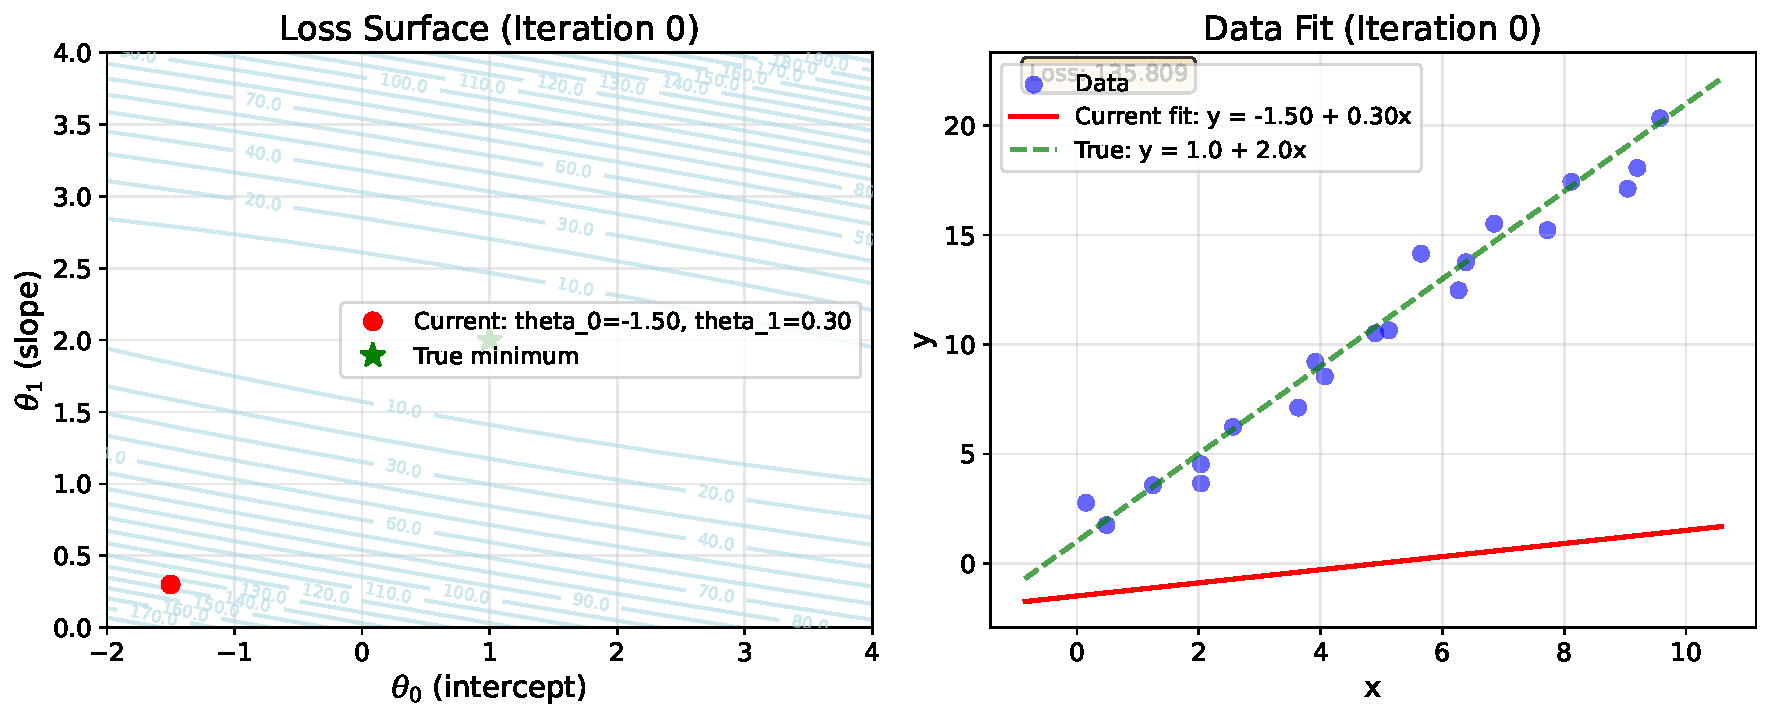
\includegraphics[width=\textwidth]{../../maths/assets/mathematical-ml/figures/gradient-descent-0.pdf}
\end{adjustbox}

\end{column}
\begin{column}{0.5\textwidth}
\begin{adjustbox}{max totalsize={\textwidth},center}
\includegraphics[width=\textwidth]{../../maths/assets/mathematical-ml/figures/contour-linreg-0.pdf}
\end{adjustbox}
\end{column}
\end{columns}




\end{frame}

\begin{frame}{Coordinate Descent : Example}
\textbf{Iteration 1}\\
\vspace{0.5cm}
INIT: $\theta_{0} = 2$ and  $\theta_{1}  = 3$\\

\vspace{0.5cm}
$\theta_1 = 3$ optimize for $\theta_{0}$\\ 
\only<2->{
\vspace{0.5cm}
$\frac{\partial \MSE}{\partial \theta_{0}} = 6\theta_0 + 24 = 0$\\
\vspace{0.5cm}
$\theta_0 = -4$


}


\end{frame}


\begin{frame}{Iteration 1}

MSE = $\frac{1}{3}(14+3\theta_{0}^{2}+14\theta_{1}^{2}-12\theta_{0}-28\theta_{1}+12\theta_{0}\theta_{1})$\\

\begin{columns}
\begin{column}{0.6\textwidth}
\begin{adjustbox}{max totalsize={\textwidth},center}
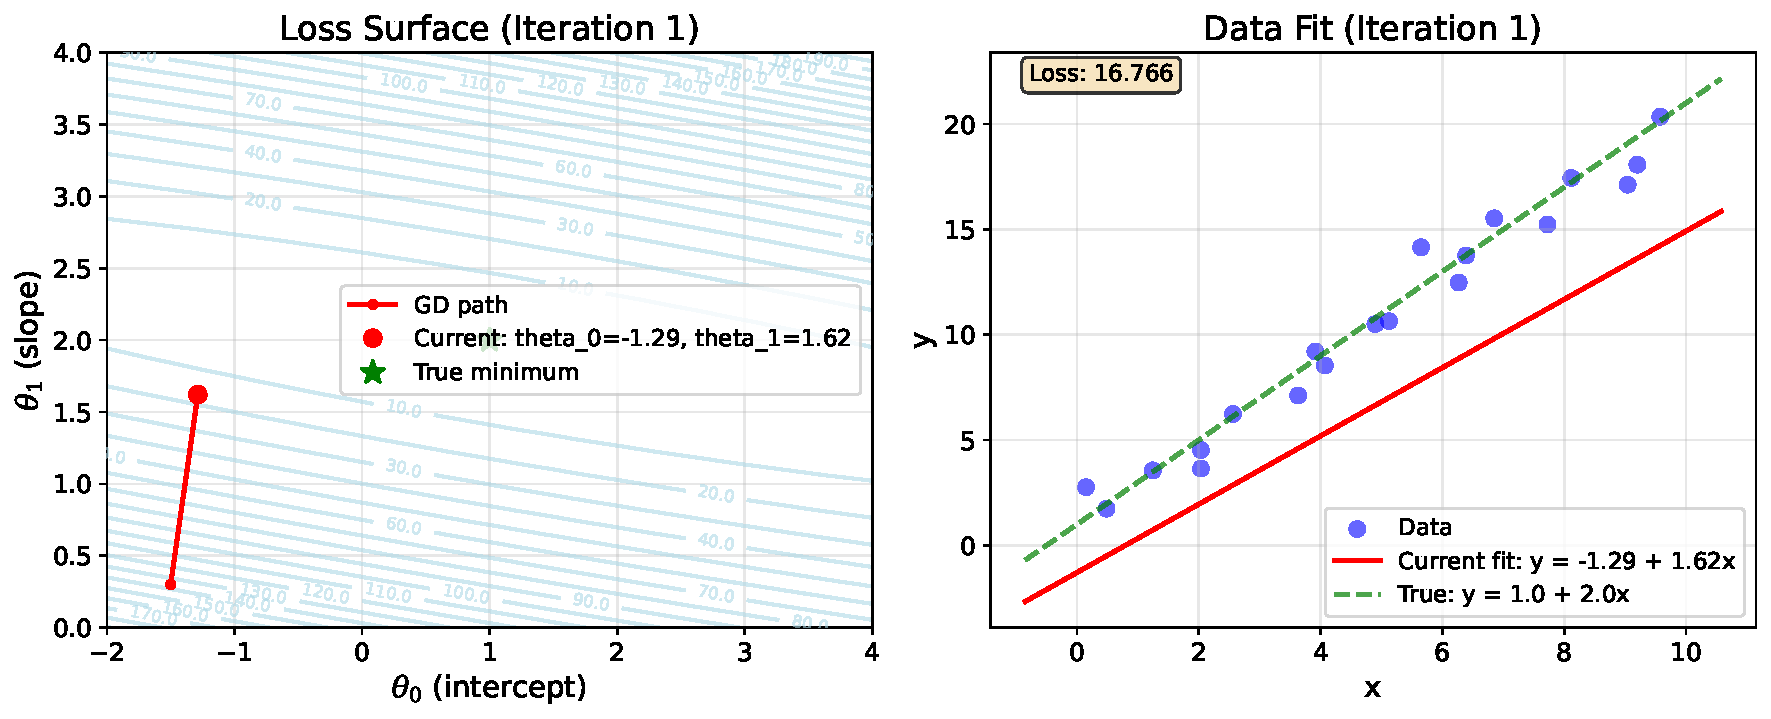
\includegraphics[width=\textwidth]{../../maths/assets/mathematical-ml/figures/gradient-descent-1.pdf}
\end{adjustbox}

\end{column}
\begin{column}{0.5\textwidth}
\begin{adjustbox}{max totalsize={\textwidth},center}
\includegraphics[width=\textwidth]{../../maths/assets/mathematical-ml/figures/contour-linreg-1.pdf}
\end{adjustbox}
\end{column}
\end{columns}


\end{frame}

\begin{frame}{Coordinate Descent : Example}
\textbf{Iteration 2}\\
\vspace{0.5cm}
INIT: $\theta_{0} = -4$ and  $\theta_{1}  = 3$\\

\vspace{0.5cm}
$\theta_0 = -4$ optimize for $\theta_{1}$\\ 
\only<2->{
\vspace{0.5cm}
$\theta_1 = 2.7$
}


\end{frame}


\begin{frame}{Iteration 2}

MSE = $\frac{1}{3}(14+3\theta_{0}^{2}+14\theta_{1}^{2}-12\theta_{0}-28\theta_{1}+12\theta_{0}\theta_{1})$\\

\begin{columns}
\begin{column}{0.6\textwidth}
\begin{adjustbox}{max totalsize={\textwidth},center}
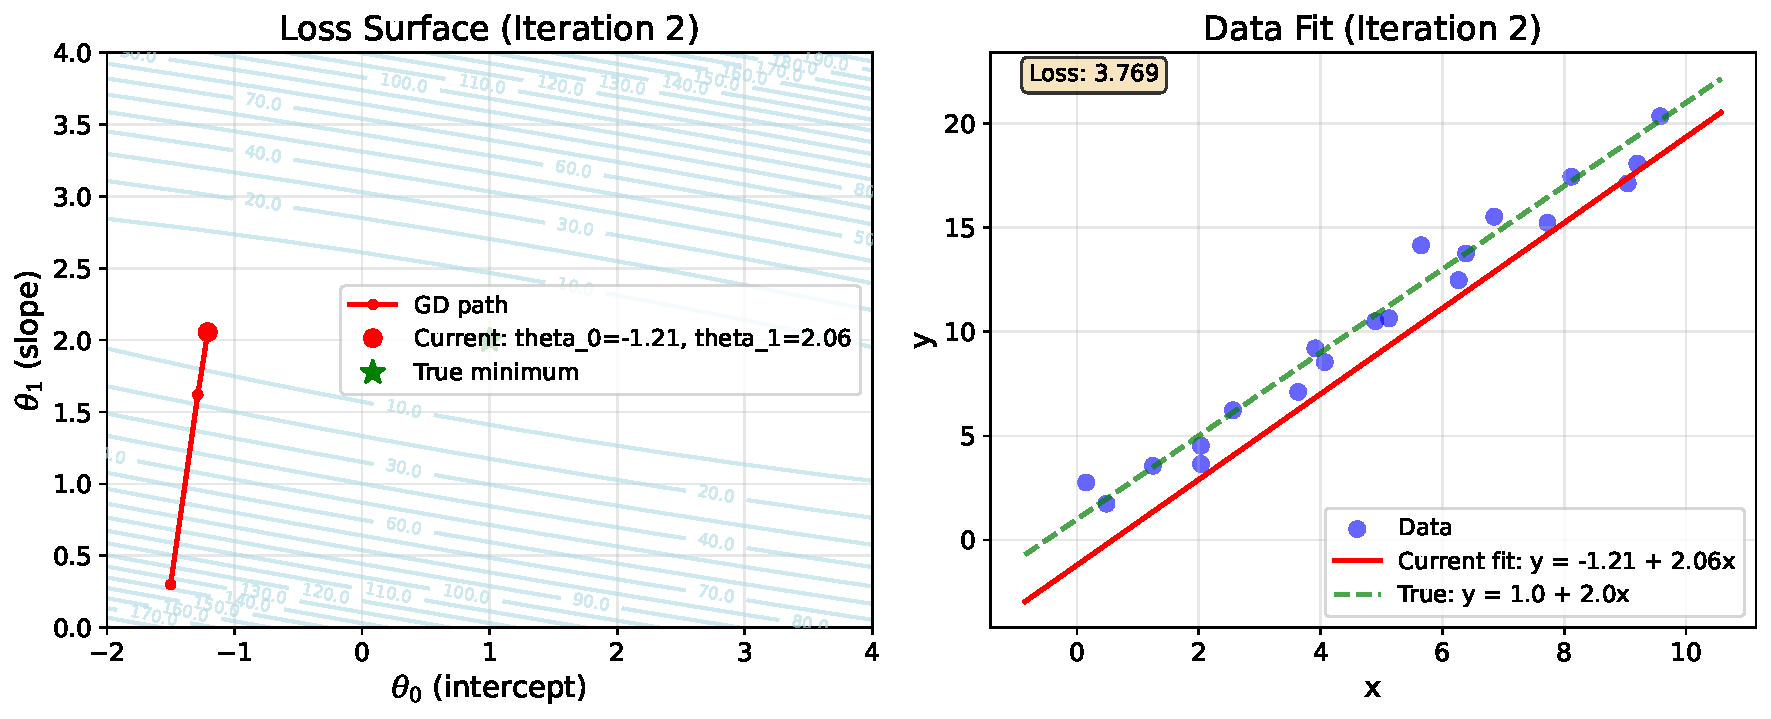
\includegraphics[width=\textwidth]{../../maths/assets/mathematical-ml/figures/gradient-descent-2.pdf}
\end{adjustbox}

\end{column}
\begin{column}{0.5\textwidth}
\begin{adjustbox}{max totalsize={\textwidth},center}
\includegraphics[width=\textwidth]{../../maths/assets/mathematical-ml/figures/contour-linreg-2.pdf}
\end{adjustbox}
\end{column}
\end{columns}


\end{frame}

\begin{frame}{Coordinate Descent : Example}
\textbf{Iteration 3}\\
\vspace{0.5cm}
INIT: $\theta_{0} = -4$ and $\theta_{1}  = 2.7$\\

\vspace{0.5cm}
$\theta_1 = 2.7$ optimize for $\theta_{0}$\\ 
\only<2->{
\vspace{0.5cm}
$\theta_0 = -3.4$
}


\end{frame}

\begin{frame}{Iteration 3}

MSE = $\frac{1}{3}(14+3\theta_{0}^{2}+14\theta_{1}^{2}-12\theta_{0}-28\theta_{1}+12\theta_{0}\theta_{1})$\\

\begin{columns}
\begin{column}{0.6\textwidth}
\begin{adjustbox}{max totalsize={\textwidth},center}
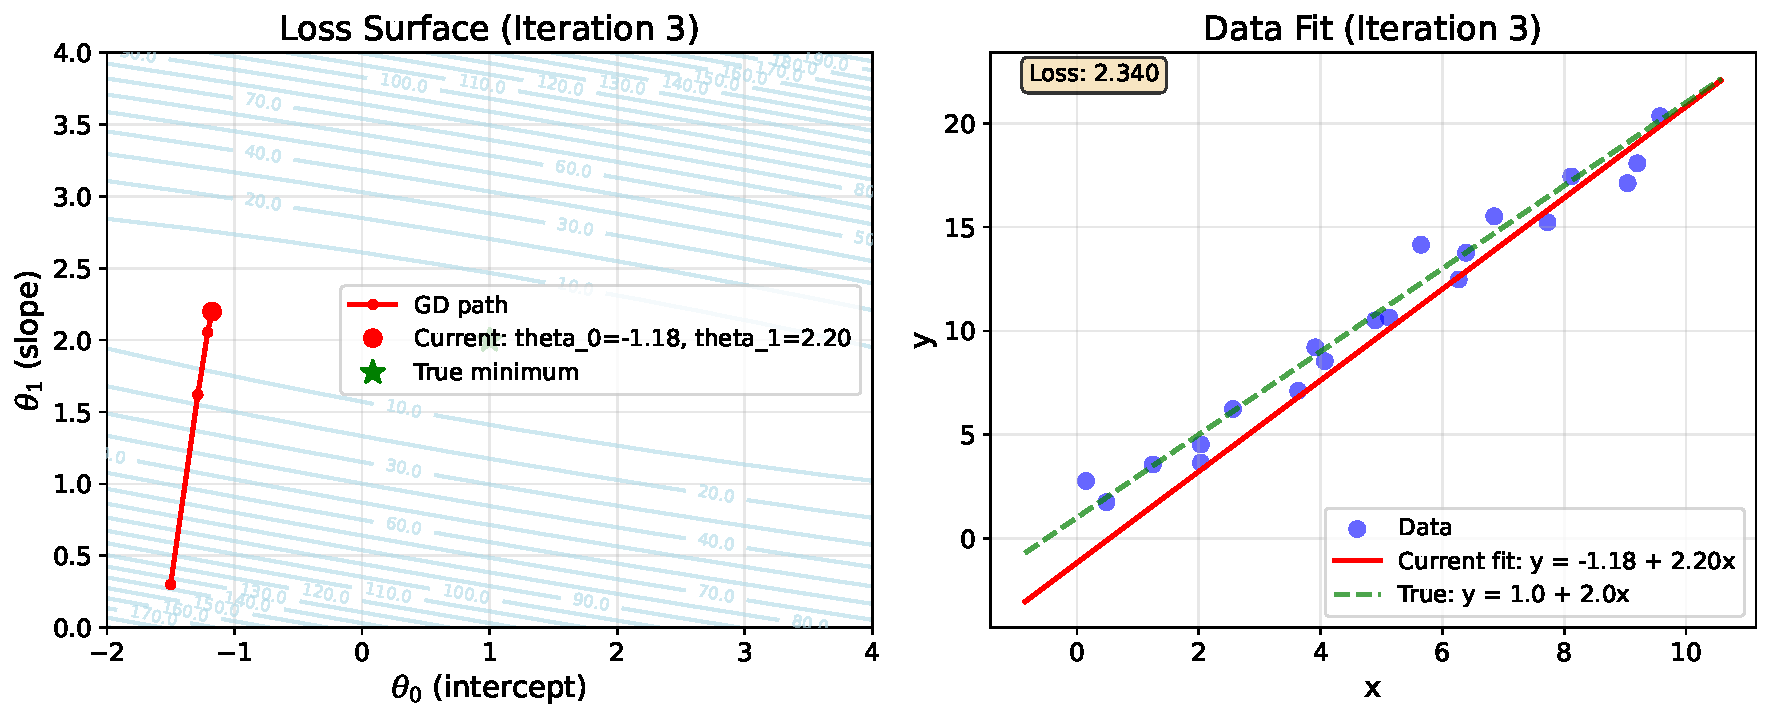
\includegraphics[width=\textwidth]{../../maths/assets/mathematical-ml/figures/gradient-descent-3.pdf}
\end{adjustbox}

\end{column}
\begin{column}{0.5\textwidth}
\begin{adjustbox}{max totalsize={\textwidth},center}
\includegraphics[width=\textwidth]{../../maths/assets/mathematical-ml/figures/contour-linreg-3.pdf}
\end{adjustbox}
\end{column}
\end{columns}


\end{frame}


%{
%\setbeamercolor{background canvas}{bg=}
%\includepdf[page=-]{coordinate-descent-fail.pdf}
%}


\begin{frame}{Coordinate Descent for Unregularised Regression}

\begin{itemize}[<+->]
	
	
	
	
	
	\item Express error as a difference of $y_{i}$ and $\hat{y_{i}}$
	\begin{equation}
	\hat{y_i} = \sum_{j=0}^{d} \theta_{j}x^{j}_{i} = \theta_{0}x_{i}^{0} + \theta_{1}x_{i}^{1} +\theta_{2}x_{i}^{2} + \ldots + \theta_{d}x_{i}^{d}
	\end{equation}
	\begin{equation}
	\epsilon_{i} = y_{i} - \hat{y_{i}} = y_{i} - \theta_{0}x_{i}^{0} - \theta_{1}x_{i}^{1} - \ldots - \theta_{d}x_{i}^{d} = y_{i} - \sum_{j=0}^{d} \theta_{j}x_{i}^{j}
	\end{equation}
	
	
	
\end{itemize}


\end{frame}



\begin{frame}{Coordinate Descent for Unregularised regression}

\[
\sum_{i=1}^{n}  \epsilon^{2}=\RSS =\sum_{i=1}^{n}\left(y_{i}-\left(\theta_{0}x_{i}^{0}+\ldots + \theta_{j} x_{i}^{j}+\theta_{d} x_{i}^{d}\right)\right)^{2}
\]
\end{frame}

\begin{frame}{Coordinate Descent for Unregularised regression}

\[
\sum_{i=1}^{n}  \epsilon^{2}=\RSS =\sum_{i=1}^{n}\left(y_{i}-\left(\theta_{0}x_{i}^{0}+\ldots + \theta_{j} x_{i}^{j}+\theta_{d} x_{i}^{d}\right)\right)^{2}
\]
\[
\frac{\partial \RSS\left(\theta_{j}\right)}{\partial \theta_{j}}= 2 \sum_{i=1}^{n}\left(y_{i}-\left(\theta_{0}x_{i}^{0}+\ldots + \theta_{j} x_{i}^{j}+\ldots \right)\right)\left(-x_{i}^{j}\right)
\]
\end{frame}

\begin{frame}{Coordinate Descent for Unregularised regression}

\[
\sum_{i=1}^{n}  \epsilon^{2}=\RSS =\sum_{i=1}^{n}\left(y_{i}-\left(\theta_{0}x_{i}^{0}+\ldots + \theta_{j} x_{i}^{j}+\theta_{d} x_{i}^{d}\right)\right)^{2}
\]
\[
\frac{\partial \RSS\left(\theta_{j}\right)}{\partial \theta_{j}}= 2 \sum_{i=1}^{n}\left(y_{i}-\left(\theta_{0}x_{i}^{0}+\ldots + \theta_{j} x_{i}^{j}+\ldots \right)\right)\left(-x_{i}^{j}\right)
\]
\[
=2\sum_{i=1}^{n}\left(y_{i}-\left(\theta_{0} x_{i}^{0}+\ldots + \theta_{d} x_{i}^{d}\right)\right)\left(-x_{i}^{j}\right)+2 \sum_{i=1}^{n} \theta_{j}(x_{i}^j)^2
\]
\pause where: $$\hat{y_{i}}^{(-j)} = \theta_{0} x_{i}^{0}+\ldots + \theta_{d} x_{i}^{d}$$ is $\hat{y}_{i}$ without $\theta_{j}$
\end{frame}

\begin{frame}{Coordinate Descent for Unregularised regression}

\[
\text{Set } \frac{\partial \RSS\left(\theta_{j}\right)}{\partial \theta_{j}}= 0
\]
\[
\theta_{j}=\sum_{i=1}^{n} \frac{\left(y_{i}-\left(\theta_{0} x_{i}^{0}+\ldots + \theta_{d} x_{i}^{d}\right)\right)\left(x_{i}^{j}\right)}{\left(x_{i}^{j}\right)^{2}}= \frac{\rho_{j}}{z_{j}}
\]
\[
\rho_{j} =\sum_{i=1}^{n} x_{i}^{j}\left(y_{i}-{\hat{y}_{i}^{(-j)}}\right) \quad \text{and} \quad z_{j}=\sum_{i=1}^{n}\left(x_{i}^{j}\right)^{2}
\]
$z_{j}$ is the squared of $\ell_2$ norm of the $j^{th}$ feature
\end{frame}

%{
%\setbeamercolor{background canvas}{bg=}
%\includepdf[page=-]{coordinate-rho.pdf}
%}




\begin{frame}{Coordinate Descent for Lasso Regression}
\[
\text{Minimise} \underbrace{\sum_{i=1}^{n} \epsilon^{2} + \delta^{2}\left\{\left|\theta_{0}\right|+\left|\theta_{1}\right|+\ldots\left|\theta_{j}\right|+\ldots |\theta_{d}|\right\}}_{\text{LASSO OBJECTIVE}}
\]
\[
\frac{\partial}{\partial \theta_{j}}(\text {LASSO OBJECTIVE})=-2 \rho_{j}+2 \theta_{j} z_{j}+\delta^{2}{\frac{\partial}{\partial \theta_{j}}}\left|\theta_{j}\right|
\]
\[
\frac{\partial}{\partial \theta_{j}}\left|\theta_{j}\right|=\left\{\begin{array}{cc}
1 & \theta_{j}>0 \\
{[-1,1]} & \theta_{j}=0 \\
-1 & \theta_{j}<0
\end{array}\right.
\]
\end{frame}

\begin{frame}{Coordinate Descent for Lasso Regression}
\begin{itemize}[<+->]
\item \textbf{Case 1: $\theta_{j}>0$}
\[
-2\rho_j+2\theta_j z_j+\delta^{2}  = 0
\]
\[
\theta_j = \frac{\rho_j - \frac{\delta^{2}}{2}}{z_{j}}
\]
\[
\rho_{j}>\frac{\delta^{2}}{2} \Rightarrow  \theta_{j} = \frac{\rho_j - \frac{\delta^{2}}{2}}{z_{j}}
\]

\item \textbf{Case 2: $\theta_{j}<0$}
\begin{equation}
\rho_{j} < \frac{\delta^{2}}{2} \Rightarrow \theta_{j} = \frac{\rho_{j}+\delta^{2} / 2}{z_{j}}
\end{equation}
\end{itemize}

\end{frame}

\begin{frame}{Coordinate Descent for Lasso Regression}
\begin{itemize}
\item \textbf{Case 3: $\theta_{j} = 0$}
\[
\frac{\partial}{\partial \theta_{j}}(\text {LASSO OBJECTIVE})=-2 \rho_{j}+2\theta_{j} z_{j}+ \delta^{2}\underbrace{{\frac{\partial}{\partial \theta_{j}}}\left|\theta_{j}\right|}_{\text{[-1,1]}}
\]
\[
\in \underbrace{[-2\rho_{j} - \delta^{2}, -2\rho_{j} + \delta^{2}]}_{\text{$\{0\}$ lies in this range}}
\]
\[
-2\rho_{j} - \delta^{2} \leq 0 \text{ and } -2\rho_{j} + \delta^{2} \geq 0
\]
\[
-\frac{\delta^{2}}{2} \leq \rho_j \leq \frac{\delta^{2}}{2}  \Rightarrow \theta_{j}=0
\]

\end{itemize}

\end{frame}
\begin{frame}{Summary of Lasso Regression}
\begin{equation}
\theta_{j} =\left[\begin{array}{ccc}
\frac{\rho_{j} + \frac{\delta^{2}}{2}}{z_{j}} & \text{if}  & \rho_{j}<-\frac{\delta^{2}}{2} \\
0 & \text{if} & -\frac{\delta^{2}}{2} \leq \rho_{j} \leq \frac{\delta^{2}}{2} \\
\frac{\rho_{j} - \frac{\delta^{2}}{2}}{z_{j}} & \text{if} & \rho_{j}>\frac{\delta^{2}}{2}
\end{array}\right]
\end{equation}

\end{frame}

%{
%\setbeamercolor{background canvas}{bg=}
%\includepdf[page=-]{coordinate-thresholding.pdf}
%}


\end{document}
